%\section{\centering Experimental Setup}
\chapter{The Standard Model of Particle Physics and Beyond}
%\chapter*{\centering Experimental Setup}
\label{ch:Theory}

Currently, the Standard Model (SM) of particle physics is the most complete theory to describe the fundamental phenomena of the universe with a finite set of laws. It classifies all known elementary particles while also describing three of the four known ways that they can interact with each other. However, there is a substantial amount of evidence that their exists physics that is not described by the SM and there are numerous theories that connect this new, beyond the SM (BSM) physics to the SM with the Higgs boson. Therefore, the production of Higgs boson pairs (HH) provides an excellent signature in particle collisions to search for new physics. This chapter will first introduce the particles that make up the SM, along with its quantum field framework and how the Higgs boson fits within it. Then HH production within the context of the SM will be discussed and finally, a few BSM theories that enhance HH production will be outlined.

%The driving goal of high energy physics has been to describe the fundamental phenomena of the universe with a finite set of laws. Currently, the Standard Model (SM) is the most complete theory to do this and with the recent discovery of the Higgs boson another prediction from the SM has been observed. However, the SM leaves many observed phenomena unexplained, for example, dark matter, the matter-antimatter asymmetry, and neutrino oscillations. To explain these phenomena, there are numerous beyond the Standard Model (BSM) theories that have been proposed and many of these theories predict new particles that interact with the Higgs boson. Therefore, the Higgs boson discovery opens new ways to search for BSM physics and this chapter will specifically focus on the productions of Higgs boson pairs (HH). First, this chapter will introduce the particles that make up the SM along with it's quantum field framework and how the Higgs boson fits within it. Then HH production within the context of the SM will be discussed and finally, how BSM theories can enhance HH production. 


\section{The Standard Model}

The SM describes all observed fundamental particles of the universe as well as their interactions according to the electromagnetic, weak, and strong forces. The fundamental particles are classified as either fermions, half-integer spin particles, or bosons, integer spin particles, where fermions make up the matter of the universe and bosons are the force carriers. All particles in the SM can be seen in Figure~\ref{fig:StandardModel}\cite{SM}.

\begin{figure}[htbp]
\begin{center}
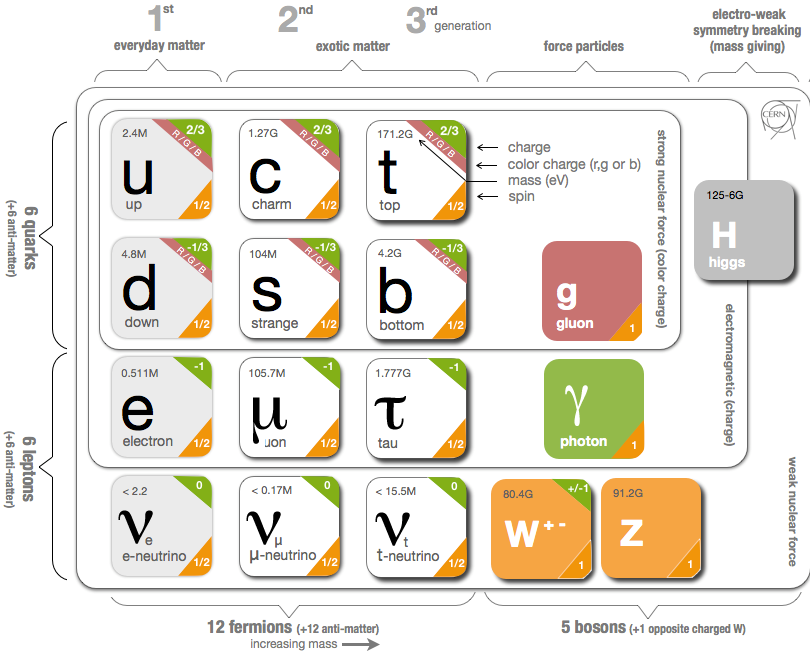
\includegraphics[width=5 in]{Theory/SM_crop2.png}
\end{center}
\caption{The quarks, leptons, and bosons that compose the Standard Model\cite{SM}.}
\label{fig:StandardModel}
\end{figure}

There are twelve fermions in the SM which are further classified into two separate groups according to how they interact: six quarks which interact through the electromagnetic, weak, and strong forces and six leptons which interact through the electromagnetic and weak forces. Also, each fermion has an antiparticle partner which has identical properties but opposite quantum numbers. The quarks and leptons are further grouped into 3 generations, where each generation contains a pair of particles. The generations of quarks contain one quark with a positive electric charge of +2/3 and one quark with a negative electric charge of -1/3. The first generation contains the positively-charged up ($u$) quark and the negatively charged down ($d$) quark, the second generation contains the positively-charged charm ($c$) quark and the negatively-charged strange ($s$) quark, and the third generation contains the positively-charged top ($t$) quark and negatively-charged bottom ($b$) quark. Each generation of quarks is identical except they have increasing mass and therefore, the second and third generation particles have short half-lives and are only observed in high energy environments. The first generation quarks are stable and make up all ordinary matter. For example, a proton contains two $u$ quarks and one $d$ quark. Since quarks interact through the strong force, they carry a color charge, analogous to electromagnetically interacting particles carrying an electromagnetic charge, and never appear individually in nature but are only found strongly bound to other quarks. This is a property called color confinement and will be discussed in more detail in Section~\ref{sec:QuantumChromo}. When quarks are bound together they form composite particles called hadrons. Hadrons can either be comprised of a quark-antiquark pair, called a meson, or three quarks, called a baryon. Protons and neutrons are examples of baryons that are found most often in the nature. 

Each generation of leptons contains a particle with a $-1$ electric charge and the corresponding electrically neutral neutrino. Since neutrinos have no electric charge they only interact via the weak force and therefore rarely interact with other particles. The first lepton generation contains the electron (e) and electron neutrino ($\nu_{e}$), the second generation contains the muon ($\mu$) and muon neutrino ($\nu_{\mu}$), and the third generation contains the tau ($\tau$) and tau neutrino ($\nu_{\tau}$). Again, increasing generations of leptons have increasing mass, except for the masses of the nuetrinos, which are unknown. Since the electrons are the lightest lepton they are stable and are the most common lepton found in the universe. 

Forces in the standard model are described through particles exchanging gauge bosons. The gauge bosons all have spin-1 and are the gluon (g), photon ($\gamma$), and $W^{\pm}$ and Z bosons. The gluon and photon are massless and mediate the strong force and electromagnetic force, respectively. The strong force binds quarks together to form nuclei and the electromagnetic force binds atoms and molecules together. There are two W bosons that carry a $+1$ electric charge ($W^{+}$) and a $-1$ electric charge ($W^{-}$), while the Z boson is electrically neutral. These three bosons are massive and mediate the weak force which is responsible for radioactive decay. Finally, the Higgs boson is a spin-0 scalar particle that generates the masses of the leptons and W and Z bosons through spontaneous symmetry breaking which will be described in Section~\ref{sec:BEHmechanism}.

The mathematical framework that describes all particles and forces of the SM is quantum field theory (QFT). The SM can be divided into two separate theories: electroweak theory, which describes the electromagnetic and weak force, and quantum chromodynamics (QCD), which describes the strong force. The particles in these theories are described as fields in space-time and a Lagrangian describes the dynamics and kinematics of the theory. The SM is also a gauge theory, a type of field theory where the Lagrangian is invariant under certain gauge groups of transformations, described by the gauge group: 

\begin{equation}
SU(3)\times SU(2)\times U(1)
\end{equation}

\noindent
where $SU(3)$ is the gauge group that describes QCD and $SU(2)\times U(1)$ describes electroweak theory. 

\subsection{Electroweak Theory}
\label{sec:ElelctroW}

Electroweak theory unifies the electromagnetic force and the weak force. This implies that at high energies, like during the early universe, these two forces manifest as a single force and it's only as the universe cooled down that they separated into two distinct forces. Therefore, the electromagnetic force can also be described by a separate QFT called quantum electrodynamics (QED). QED is invariant under $U(1)_{em}$, which is defined by the gauge transformation

\begin{equation}
\psi(x)\rightarrow e^{i\alpha(x)Q}\psi(x)
\end{equation}

\noindent
where $\alpha(x)$ is an arbitrary function of space and time and $Q$, the electric charge, is the generator for the group. The Lagrangian for this transformation can be derived by keeping the Dirac Lagrangian invariant under the transformation. This leads to

\begin{equation}
\mathcal{L}= \bar{\psi}(i\gamma^{\mu}\partial_{\mu} - m)\psi + e\bar{\psi}\gamma^{\mu}A_{\mu}\psi - \frac{1}{4}F_{\mu\nu}F^{\mu\nu}
\end{equation}

\noindent
where the first term represents the free propagation of a particle, $\psi$. The second term describes the interactions between the particle and a photon field, $A_{\mu}$, and is proportional to the electromagnetic coupling constant, $e$. The final term represents the kinetic energy of the photon field, where $F_{\mu\nu}=\partial_{\mu}A_{\nu}-\partial_{\nu}A_{\mu}$. The photon is required to be massless because the addition of a mass term, $\frac{1}{2}m^{2}A_{\mu}A^{\mu}$, would break gauge invariance. 

To incorporate the weak force, a field theory is built that is invariant under $SU(2)_{L}\times U(1)_{Y}$. This gauge group is represented by the following transformations

%Electroweak theory is a chiral theory, which means that left-handed and right handed particles transform differently by the gauge transformation. The “handedness” of a particle is defined by it’s helicity, which is the dot product of the momentum and spin unit vectors, so a left-handed particle has helicity $-1$ and a right-handed particle has helicity $+1$. The gauge transformation for the two handedness particles is

%The $L$ subscript indicates that weak isospin only couples to left-handed fermions.

\begin{align}
\begin{split}
&\chi_{L}\rightarrow e^{i\alpha (x)\cdot I + i\beta (x)Y}\chi_{L},
\\
&\psi_{R} \rightarrow e^{i\beta(x)Y}\psi_{R}
\end{split}
\end{align}

\noindent
where these two transformations depend on the "handedness," or helicity, of a particle. The helicity is the dot product of the momentum and spin unit vectors, so a left-handed particle has helicity $-1$ and a right-handed particle has helicity $+1$. In the above transformations, $I$ is the generator for $SU(2)_{L}$ and $I_{i}=\frac{\sigma_{i}}{2}$, where $\sigma_{i}$ are the standard Pauli matrices. The hypercharge, $Y$, is the generator of $U(1)_{Y}$ and represents one of the charges of the electroweak interaction. The other charge is $I_{3}$, called weak isospin. Left-handed fermions, $\chi_{L}$, form isospin doublets with weak isospin $\pm\frac{1}{2}$ and right-handed fermions, $\psi_{R}$, form isosinglets with weak isospin $0$. These generators are related to the generator of QED by

\begin{equation}
Q=I_{3}+\frac{Y}{2}.
\end{equation}

\noindent
The electroweak Lagrangian is

\begin{equation}
\begin{split}
&\mathcal{L}=-\frac{1}{4}W^{i}_{\mu\nu}\cdot W_{i}^{\mu\nu} -\frac{1}{4}B_{\mu\nu}B^{\mu\nu} \\
& +\chi_{L}\gamma^{\mu}(i\partial_{\mu}-\frac{g}{2}\sigma_{i}W^{i}_{\mu}-g^{\prime}\frac{Y}{2}B_{\mu})\chi_{L} \\
& + \psi_{R}\gamma^{\mu}(i\partial_{\mu}-g^{\prime}\frac{Y}{2}B_{\mu})\psi_{R}
\end{split}
\end{equation}

\noindent
where $W^{i}_{\mu\nu} \equiv \partial_{\mu}W^{i}_{\mu}-\partial_{\nu}W^{i}_{\mu} -g\epsilon_{ijk}W^{j}_{\mu}W^{k}_{\nu}$, $B_{\mu\nu}\equiv \partial_{\mu}B_{\nu}-\partial_{\nu}B_{\mu}$, and $g$ and $g^{\prime}$ are the coupling constants for $SU(2)_{L}$ and $U(1)_{Y}$, respectively. The mediators are the three massless $W^{i}$ bosons which form a weak isospin triplet and a massless $B^{0}$ boson which forms a weak isospin singlet. These massless bosons become the massive $W^{\pm}$ and $Z$ bosons and the massless photon through the Brout-Englert-Higgs mechanism which will be described in more detail in Section~\ref{sec:BEHmechanism}. The large mass of the $W^{\pm}$ and $Z$ bosons causes them to be short-lived particles and therefore, the weak force is a short range force. Since the photon is massless, the electromagnetic force is a long-range interaction.



%It’s important to note that there are no mass terms in this Lagrangian since that would break the gauge symmetry. However, we know this I unphysical since most particles do have mass. There must be a mechanism to introduce mass terms into the Lagrangian without breaking gauge invariance. This mechanism is the Brout-Englert-Higgs mechanism which uses spontaneous symmetry breaking to add mass terms to the Lagrangian. This mechanism will be discussed in more detail in Section~\ref{sec:BEHmechanism}. This symmetry breaking causes the $W^{3}_{\mu}$ and $B_{\mu}$ fields to mix to form the massive Z boson and massless photon through the Weinberg mixing angle, $\theta_{W}$:


%\begin{align}
%\begin{split}
%A_{\mu}=B_{\mu}\mathrm{cos}\theta_{W}+W^{3}_{\mu}\mathrm{sin}\theta_{W},
%\\
%Z_{\mu}=-B_{\mu}\mathrm{sin}\theta_{W} + W^{3}_{\mu}\mathrm{cos}\theta_{W}
%\end{split}
%\end{align}

%\noindent
%The $W^{1}_{\mu}$ and $W^{2}_{\mu}$ mix to form the massive $W^{\pm}$ bosons through the following relation

%\begin{equation}
%W^{\pm}_{\mu}=\frac{1}{\sqrt{2}}(W^{1}_{\mu}\mp W^{2}_{\mu})
%\end{equation}

%\noindent
%These systems of equations can be rearranged and shown that

%\begin{equation}
%\frac{M_{W}}{M_{Z}}=\mathrm{cos}\theta_{W}
%\end{equation} 

%\noindent
%which implies that $M_{Z}>M_{W}$.

\subsection{Quantum Chromodynamics}
\label{sec:QuantumChromo}

The strong force is described by QCD, a field theory that is invariant under the $SU(3)$ gauge group. Particles that interact through this force can carry three types of color charge, ``red,'' ``green,'' or ``blue,'' which are represented as rotations according to $SU(3)$. This gauge group is represented by the gauge transformation

\begin{equation}
\psi(x)\rightarrow U\psi(x)\equiv e^{i\alpha_{a}T_{a}}\psi(x)
\end{equation}

\noindent
where $U$ is a $3\times3$ unitary matrix and $T_{a}$, where $a=1,...8$, are are the group generators which are hermitian matrices and satisfy the relation

\begin{equation}
[T_{a},T_{b}] = if_{abc}T_{c}
\end{equation}

\noindent
where $f_{abc}$ is the structure constant of the $SU(3)$ group. To remain invariant under this transformation, the QCD Lagrangian is written as

%\begin{equation}
%\mathcal{L}= \bar{q}(i\gamma^{\mu}D_{\mu} - m)q - \frac{1}{4}G^{\alpha}_{\mu\nu}G^{\mu\nu}_{\alpha}
%\end{equation}

\begin{equation}
\mathcal{L}= \bar{\psi}(i\gamma^{\mu}\partial_{\mu} - m)\psi - g(\bar{\psi}\gamma^{\mu}T_{a}\psi)A^{a}_{\mu} - \frac{1}{4}G^{\alpha}_{\mu\nu}G^{\mu\nu}_{\alpha}
\end{equation}
 
\noindent
which has a very similar form to the QED Lagrangian. The first term describes the free propagation of a quark and the second term represents the interactions between a quark and the vector gluon field, $A^{\alpha}_{\mu}$, and is proportional to the strong coupling constant, $g$. The final term represents the kinetic energy of the gluon field, where $G^{\alpha}_{\mu\nu}=\partial_{\mu}A^{\alpha}_{\mu} - \partial_{\nu}A^{\alpha}_{\nu} - gf_{abc}A^{b}_{\mu}A^{c}_{\nu}$. Therefore, there are cubic and quartic self-interactions of gluon fields represented in this term.

These self-interaction terms are the key difference between QCD and QED and give rise to a couple phenomena that are unique to QCD. One of these features is called asymptotic freedom, which states that the interaction between two quarks becomes smaller as the distance decreases. This can be explained by comparing the QCD and QED equivalents. In QED, a lone particle with an electromagnetic charge in a vacuum causes the vacuum to become polarized and therefore, the charge of the particle appears smaller as the distance from the particle increases. This is called the screening effect. The same effect happens in QCD when a particle with color charge sits alone in a vacuum. However, there is an additional antiscreening effect caused by the gluon self-interaction that overpowers the screening effect. Therefore, the further the distance from a color charge the larger the charge appears. This means that the coupling constant decreases as the distance decreases or the momentum scale increases.

Another property of QCD, called color confinement, is that no free particle can have a non-neutral color charge. This means that quarks only exist bound together in hadrons and when they try to separate in high energy collisions they behave like a spring, where the energy builds up between them as they separate. Eventually, this energy is large enough to produce a quark-antiquark pair in a process called hadronization. 


\section{The Brout-Englert-Higgs Mechanism}
\label{sec:BEHmechanism}

The Brout-Englert-Higgs (BEH) mechanism~\cite{BEmechanism,Hmechanism} was proposed to fix the discrepancy between the electroweak theory and what is observed in reality. As stated in Section~\ref{sec:ElelctroW}, electroweak theory predicts four bosons that are required to be massless due to gauge invariance but only one massless boson and three massive ones exist. The BEH mechanism generates the masses for these bosons while also generating the masses of the fermions by spontaneously breaking the $SU(2)_{L}\times U(1)_{Y}$ symmetry. This is done by introducing a complex scalar field that is a doublet of $SU(2)$

\begin{equation}
\Phi = 
\begin{pmatrix}
\phi^{+}\\
\phi^{0}
\end{pmatrix}
\end{equation}

\noindent
and it's corresponding Lagrangian

\begin{equation}
\label{eq:HiggsLag}
\mathcal{L} = (D_{\mu}\Phi)^{\dag}(D^{\mu}\Phi) - V(\Phi^{\dag}\Phi)
\end{equation}

\noindent
where $D_{\mu}\equiv \partial_{\mu} - ig\frac{\sigma_{i}}{2}W^{i}_{\mu} - \frac{i}{2}g^{\prime}B_{\mu}$. This Lagrangian is invariant under $SU(2)_{L}\times U(1)_{Y}$ transformations, so it can be added to the electroweak Lagrangian. The potential, $V(\Phi^{\dag}\Phi)$, is defined as

\begin{equation}
V(\Phi^{\dag}\Phi)=\mu^{2}\Phi^{\dag}\Phi+\lambda(\Phi^{\dag}\Phi)^{2}
\end{equation}

\noindent
where $\lambda>0$ implies that the potential has a minimum. In QFT, the ground state is the vacuum and is found by minimizing the potential, which gives the vacuum expectation value (VEV) of $\Phi$. Taking $\mu^{2}>0$ causes the potential to only have a minimum at $\Phi^{\dag}\Phi=0$ and no spontaneous symmetry breaking can occur. Therefore, $\mu^{2}$ is required to be less than zero and the minimum of the potential occurs when $\Phi^{\dag}\Phi=-\frac{\mu^{2}}{2\lambda}$. This means there are a degenerate set of ground states with a VEV, $v$, equal to $\sqrt{-\frac{\mu^{2}}{2\lambda}}$ and choosing a specific ground state leads to spontaneous symmetry breaking of $SU(2)_{L}\times U(1)_{Y}$. Selecting 

\begin{equation}
\Phi_{0} =
\begin{pmatrix}
0\\
v
\end{pmatrix}
\end{equation}

\noindent
as a ground state allows the scalar field to be invariant under the $U(1)_{em}$ symmetry group since the VEV is only given to the neutral component of $\Phi$. Expanding $\Phi$ around the minimum, $v$, gives

\begin{equation}
%\label{eq:GroundSt}
\Phi(x) = \frac{1}{\sqrt{2}} e^{i\sigma_{i}\theta^{i}(x)/\nu}
\begin{pmatrix}
0\\
\nu+H(x)
\end{pmatrix}
\end{equation}

\noindent
where a new Higgs field, $H(x)$, and three Goldstone bosons, $\theta^{i}(x)$, have been introduced. These Goldstone bosons are predicted by the Goldstone theorem~\cite{GoldstoneThm}, which states that massless scalars occur whenever a continuous symmetry is spontaneously broken. Since the Lagrangian is locally $SU(2)_{L}$ invariant, the three $\theta^{i}(x)$ fields can be rotated away making these massless excitations unphysical and leaving the ground state as

\begin{equation}
\label{eq:GroundSt}
\Phi(x) = \frac{1}{\sqrt{2}}
\begin{pmatrix}
0\\
\nu+H(x)
\end{pmatrix}.
\end{equation}

\noindent
When this ground state is substituted into the Lagrangian in Eq.~\ref{eq:HiggsLag}, the kinetic piece takes the form

\begin{equation}
\frac{1}{2}\partial_{\mu}H\partial^{\mu}H+(v + H)^{2}\Big\{\frac{g^{2}}{4}W_{\mu}^{+}W^{\mu-}+\frac{1}{8}(g^{2}+g^{\prime 2})Z_{\mu}Z^{\mu}\Big\}
\end{equation}

\noindent
where the physical gauge fields are defined in terms of the massless mediators as:

\begin{align}
%\begin{split}
&W^{\pm}_{\mu}=\frac{1}{\sqrt{2}}(W^{1}_{\mu}\mp W^{2}_{\mu}),
\\
&Z_{\mu}=\frac{1}{\sqrt{g^{2}+g^{\prime2}}}(gW_{\mu}^{3}-g^{\prime}B_{\mu}),
\\
&A_{\mu}=\frac{1}{\sqrt{g^{2}+g^{\prime2}}}(gW_{\mu}^{3}+g^{\prime}B_{\mu}).
%\end{split}
\end{align}

\noindent
Therefore, $A_{\mu}$ remains massless, corresponding to the massless $\gamma$, and the $W^{\pm}$ and $Z$ fields acquire masses of $\frac{1}{2}v g$ and $\frac{1}{2}v\sqrt{g^{2}+g^{\prime 2}}$, respectively. The three massive gauge bosons have absorbed a degree of freedom from the Goldstone bosons and acquired mass in the process.

The remaining portion of the Lagrangian from Eq.~\ref{eq:HiggsLag} after the substitution of the chosen ground state describes the real, scalar Higgs field and is written as

\begin{equation}
\label{eq:HiggsLag}
\mathcal{L}=\frac{1}{2}\partial_{\mu}H\partial^{\mu}H -\lambda v^{2}H^{2}-\lambda v H^{3}-\frac{\lambda}{4}H^{4}.
\end{equation}

\noindent
From this equation, the Higgs field has mass, $m_{H}=2\lambda v^{2}$, which can only be determined experimentally since $\lambda$ is a free parameter. Another feature in this equation of motion is that there are two Higgs self-coupling terms completely determined by the mass of the Higgs and the VEV. Therefore, measuring the self-coupling is a crucial test of electroweak symmetry breaking.

Finally, the masses of fermions from the electroweak theory need to be addressed. This is done by introducing the $SU(2)_{L}\times U(1)_{Y}$ invariant Yukawa Lagrangian

\begin{equation}
\mathcal{L}= -G_{f}(\bar{\chi}_{L}\Phi\phi_{R} + \bar{\phi}_{R}\Phi\chi_{L}) - G_{f^{\prime}}(\bar{\chi}_{L}\widetilde{\Phi}\phi_{R} + \bar{\phi}_{R}\widetilde{\Phi}\chi_{L})
\end{equation}

\noindent
where the conjugate of $\Phi$, $\widetilde{\Phi}=-i\sigma_{2}\Phi^{\ast}$, has been introduced. Substituting the same ground state as before from Eq.~\ref{eq:GroundSt}, the Lagrangian becomes

%\begin{equation}
%\mathcal{L}=-\frac{G_{e}}{\sqrt{2}}(v+H)\bar{e}_{L}e_{R} + ...
%\end{equation}

\begin{equation}
\mathcal{L}=-\frac{G_{f}}{\sqrt{2}}(v+H)(\bar{\psi}_{L}\psi_{R} + \bar{\psi}_{R}\psi_{L})
\end{equation}


\noindent
where this has been written for the general fermion field, $\psi$. Therefore, the mass of a fermion is equal to $\frac{G_{f}v}{\sqrt{2}}$. There is also an additional term that couples the Higgs scalar to a fermion and changes the chirality of the fermion. The coupling is proportional to the mass of the fermion and is a free parameter in the SM. 


\section{The Higgs Boson}

In 2012, nearly 40 years after the BEH mechanism was proposed, the Higgs boson was discovered by the CMS and ATLAS Collaborations at the LHC~\cite{ATLASHiggs, CMSHiggs}. The discovery was made by combining five different Higgs decay modes, $\gamma\gamma$, $ZZ$, $W^{+}W^{-}$, $\tau^{+}\tau^{-}$, and $b\bar{b}$, from $\sqrt{s}=7$ and $8$ TeV data. Despite having smaller branching fractions, which can be seen in Table~\ref{tab:HiggsBR}, the two leading contributions to the discovery were the $\gamma\gamma$ and $ZZ\rightarrow 4l$ channels due to the clean signature of these decays. The invariant mass distributions for these two channels from the CMS experiment are shown in Figure~\ref{fig:HiggsMeasurement} and a clear bump in the data can be seen at $125$ GeV. The CMS and ATLAS experiments combined to measure the mass of the Higgs~\cite{CombinedHiggs} as

\begin{equation}
m_{H}=125.09\pm 0.21(stat.)\pm 0.11(syst) ~\mathrm{GeV}.
\end{equation}

\noindent
This discovery was a great success for the SM and many properties of the new scalar boson were measured~\cite{ATLASHiggsProperties, CMSHiggsProperties} to confirm that it is consistent with the SM Higgs boson. For example, the spin and parity of the particle, the total decay width, the coupling strengths to fermions and vector bosons, and the differential production cross sections have all been probed and have thus far been shown to agree with SM predictions~\cite{HiggsProperties}. The CMS and ATLAS combined measurements of the Higgs coupling strengths can be seen in Figure~\ref{fig:HiggsCouplingMeasurement}. 

One of the remaining Higgs measurements is of the Higgs self-coupling, $\lambda_{\mathrm{HHH}}$. This is a crucial test to verify that the discovered Higgs is represented by the Lagrangian in Eq.~\ref{eq:HiggsLag}. The Higgs self-coupling can only be directly accessed by measuring Higgs pair production (HH) and therefore measuring HH production is an essential step to verify the BEH mechanism.


%\begin{figure}
%\begin{minipage}[b]{0.5\textwidth}
%	\centering
%	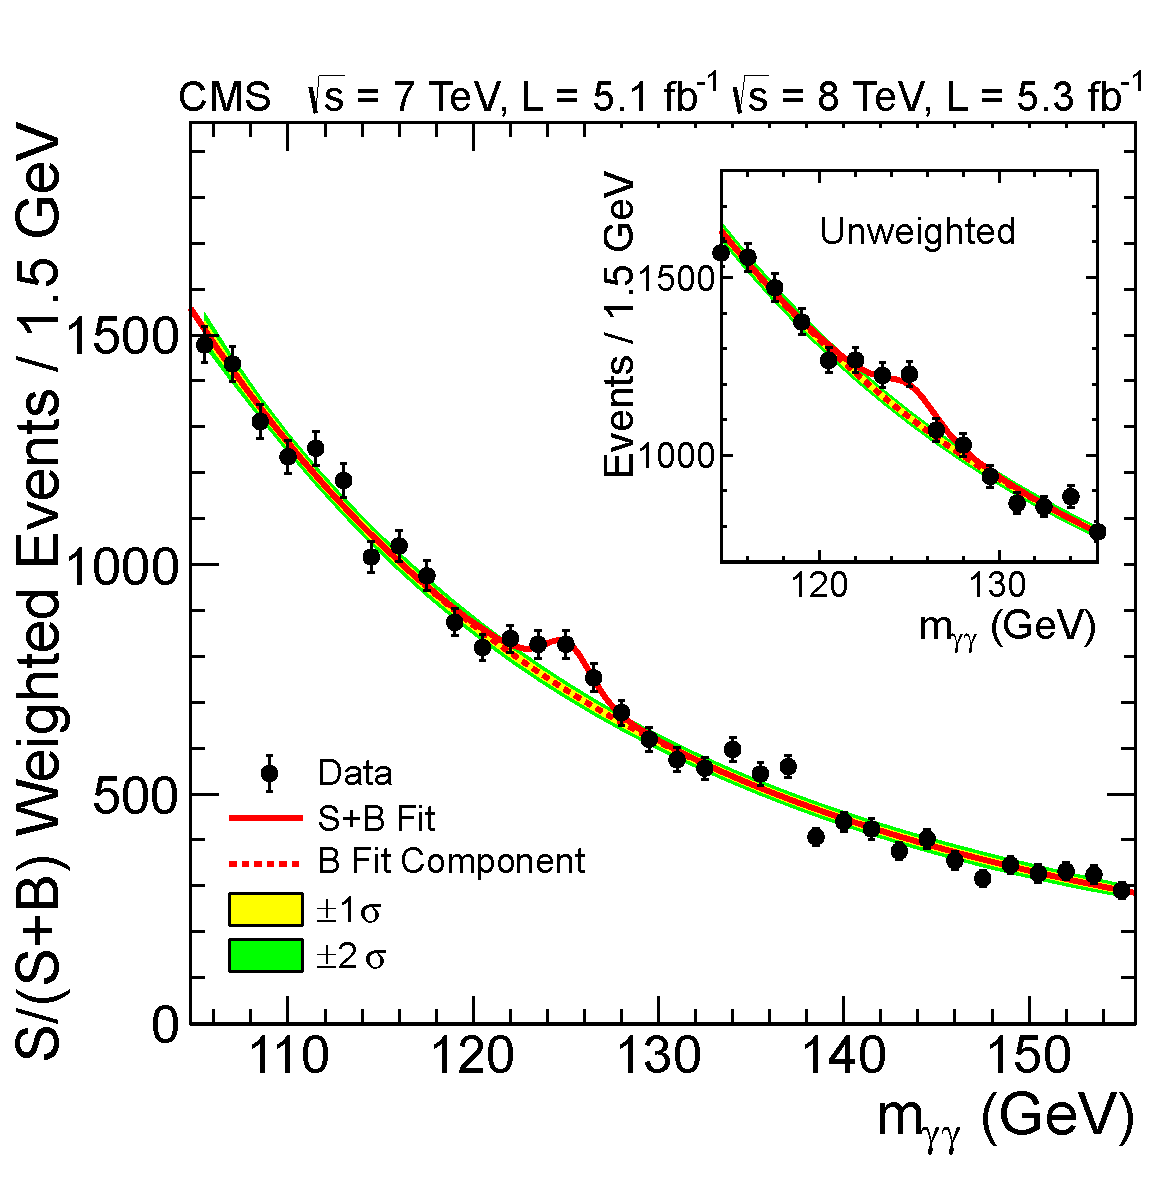
\includegraphics[width=\linewidth]{Theory/sbweightedmassunweightedinset1_5GeV.pdf}
%\end{minipage}
%\hspace{0.5cm}
%\begin{minipage}[b]{0.5\textwidth}
%	\centering
%	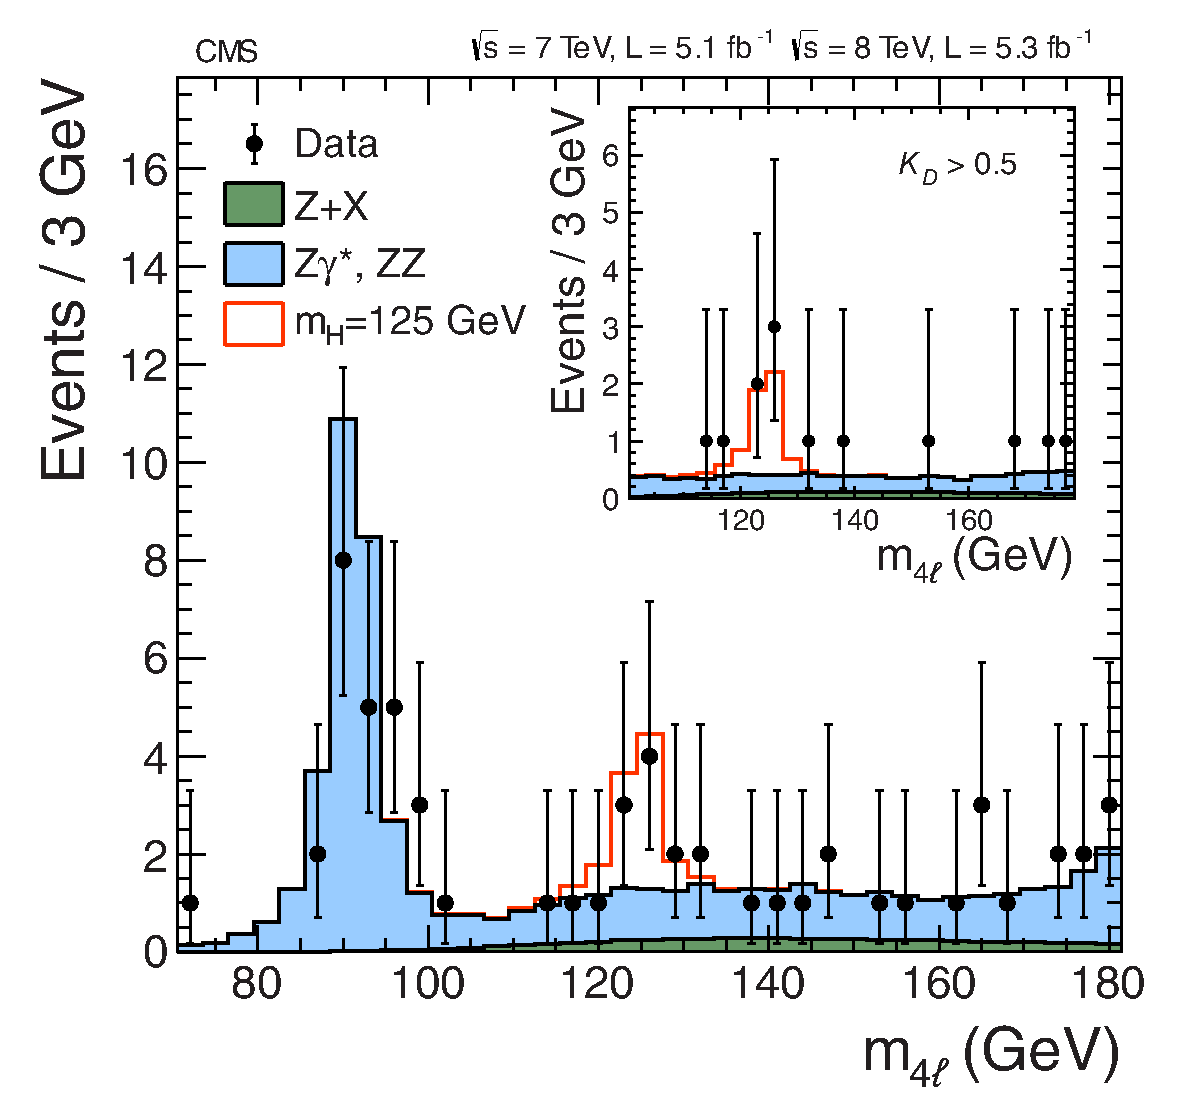
\includegraphics[width=\linewidth]{Theory/H4l_mass_v3.pdf}
%\end{minipage}
%\caption{(Left) The invariant diphoton mass distribution with each event weighted by the $\frac{S}{S+B}$ value of its category. The lines represent the fitted background and signal, and the colored bands represent the $\pm1$ and $\pm2$ standard deviation uncertainties in the background estimate. (Right) Distribtuon of the four-lepton invariant mass for the $ZZ\rightarrow 4l$ analysis. The points represent the data, the filled histograms represent the background, and the open histogram show the signal expectation for a Higgs boson of mass $m_{H}=125$ GeV~\cite{CMSHiggs}.}
%\label{fig:HiggsMeasurement}
%\end{figure}

\begin{figure}[h!]
 
\begin{subfigure}{0.5\textwidth}
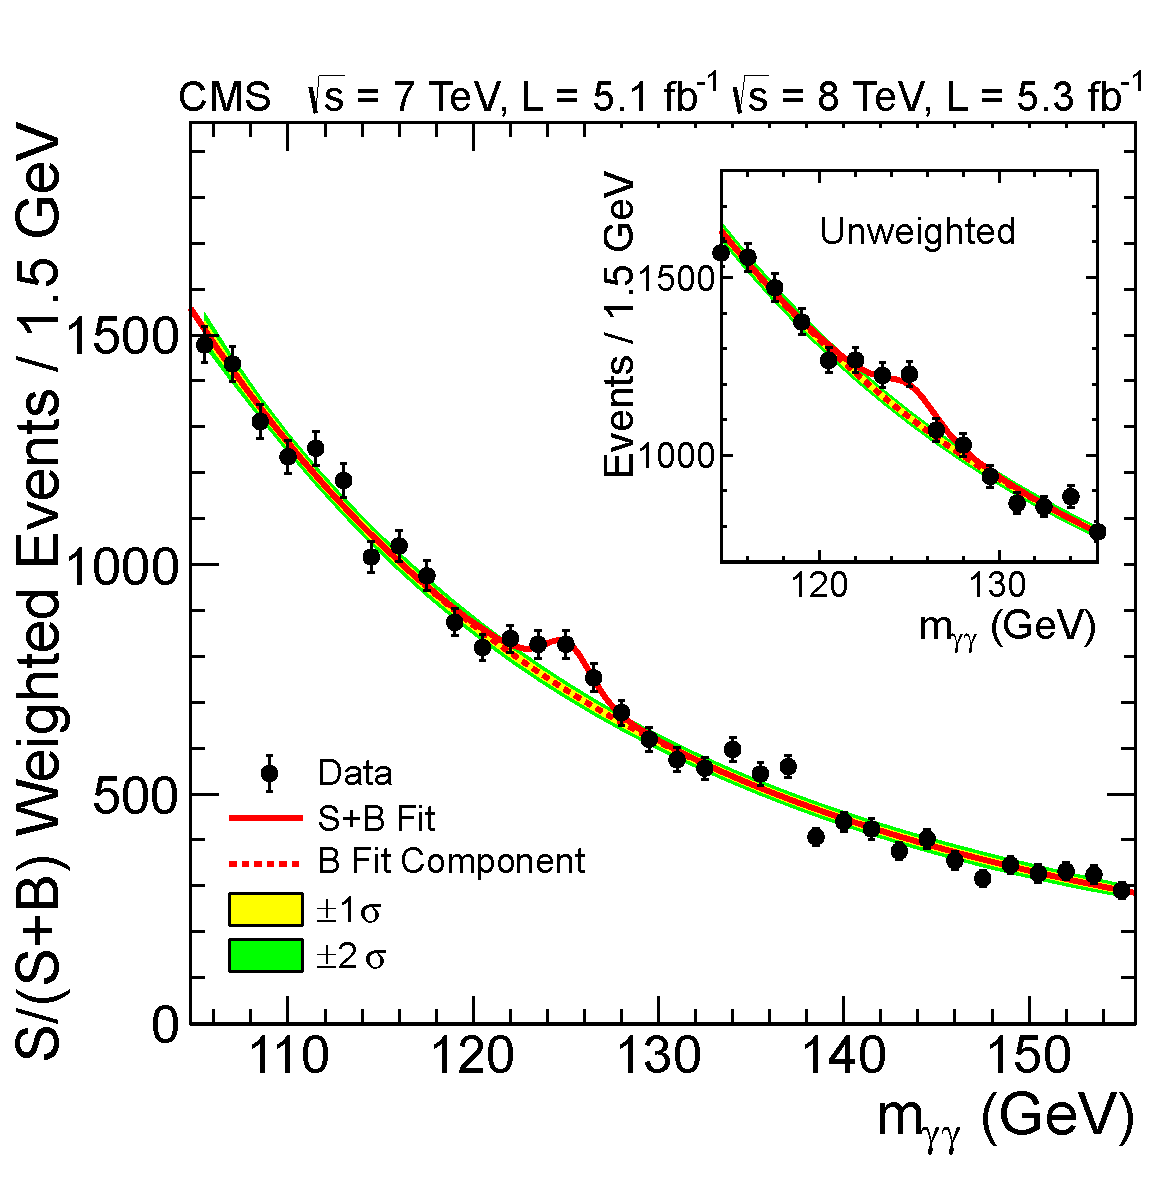
\includegraphics[width=0.9\linewidth, height=8cm]{Theory/sbweightedmassunweightedinset1_5GeV.pdf} 
\end{subfigure}
\begin{subfigure}{0.5\textwidth}
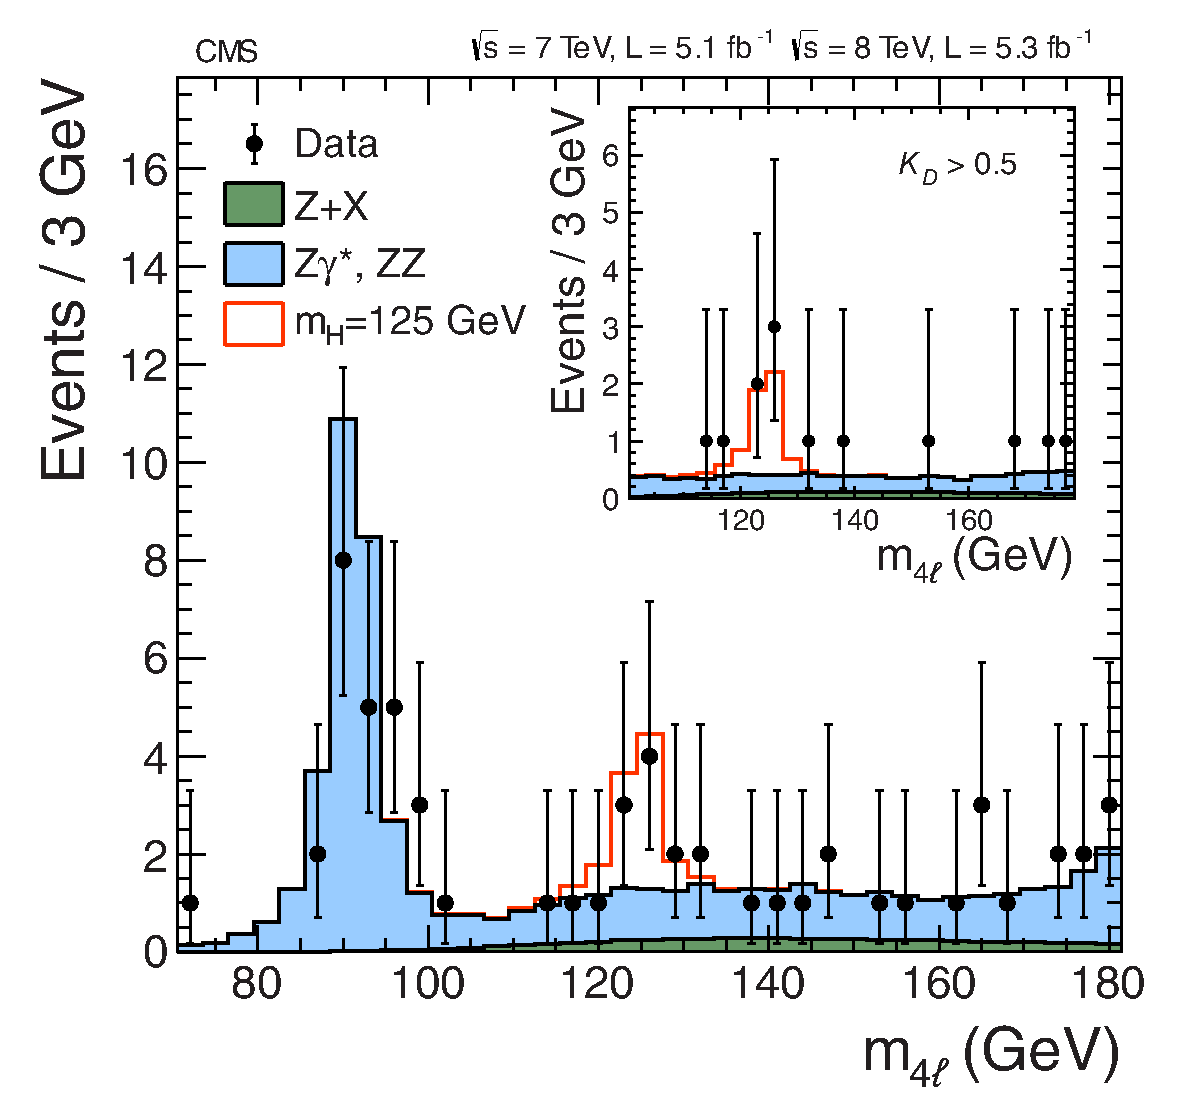
\includegraphics[width=0.9\linewidth, height=7.5cm]{Theory/H4l_mass_v3.pdf}
\end{subfigure}
 
\caption{(Left) The invariant diphoton mass distribution with each event weighted by the $\frac{S}{S+B}$ value of its category. The lines represent the fitted background and signal, and the colored bands represent the $\pm1$ and $\pm2$ standard deviation uncertainties in the background estimate. (Right) Distribtuon of the four-lepton invariant mass for the $ZZ\rightarrow 4l$ analysis. The points represent the data, the filled histograms represent the background, and the open histogram show the signal expectation for a Higgs boson of mass $m_{H}=125$ GeV~\cite{CMSHiggs}.}
\label{fig:HiggsMeasurement}
\end{figure}

{\renewcommand{\arraystretch}{1.5}
\begin{table}[h!]
\begin{center}
    \begin{tabular}{c c}
    \hline
    \hline
    Decay mode &  Branching fraction ($\%$) \\
    \hline
    $\mathrm{b\bar{b}}$ &  $58.4^{+3.2}_{-3.3}$\\
    $\mathrm{W^{+}W^{-}}$ & $21.4^{+4.3}_{-4.2}$ \\
    gg & $8.19^{+5.1}_{-5.1}$ \\
    $\tau^{+}\tau^{-}$ & $6.27^{+5.7}_{-5.7}$  \\
    $\mathrm{c\bar{c}}$ & $2.89^{+5.5}_{-2.0}$ \\
    ZZ & $2.62^{+4.3}_{-4.1}$ \\
    $\gamma\gamma$ & $0.227^{+5.0}_{-4.9}$ \\
    $\mathrm{Z}\gamma$ & $0.153^{+9.0}_{-8.9}$ \\
    $\mu^{+}\mu^{-}$ & $0.0218^{+6.0}_{-5.9}$ \\
    \hline
    \hline
    \end{tabular}
    \caption{Branching fractions for the Higgs boson with a mass of $125$ GeV. The relative uncertainties are calculated from theoretical predictions that depend on the uncertainties of $\alpha_{s}$, the quark masses, and the Higgs boson partial width.}\label{tab:HiggsBR}
\end{center}
\end{table}}


% and the HH production cross section at $\sqrt{s}=13$ TeV is ${\sim}35$ fb, which is about 1000 times smaller than SM Higgs production cross sections. Therefore, 
\begin{figure}[h!]
 \centering
 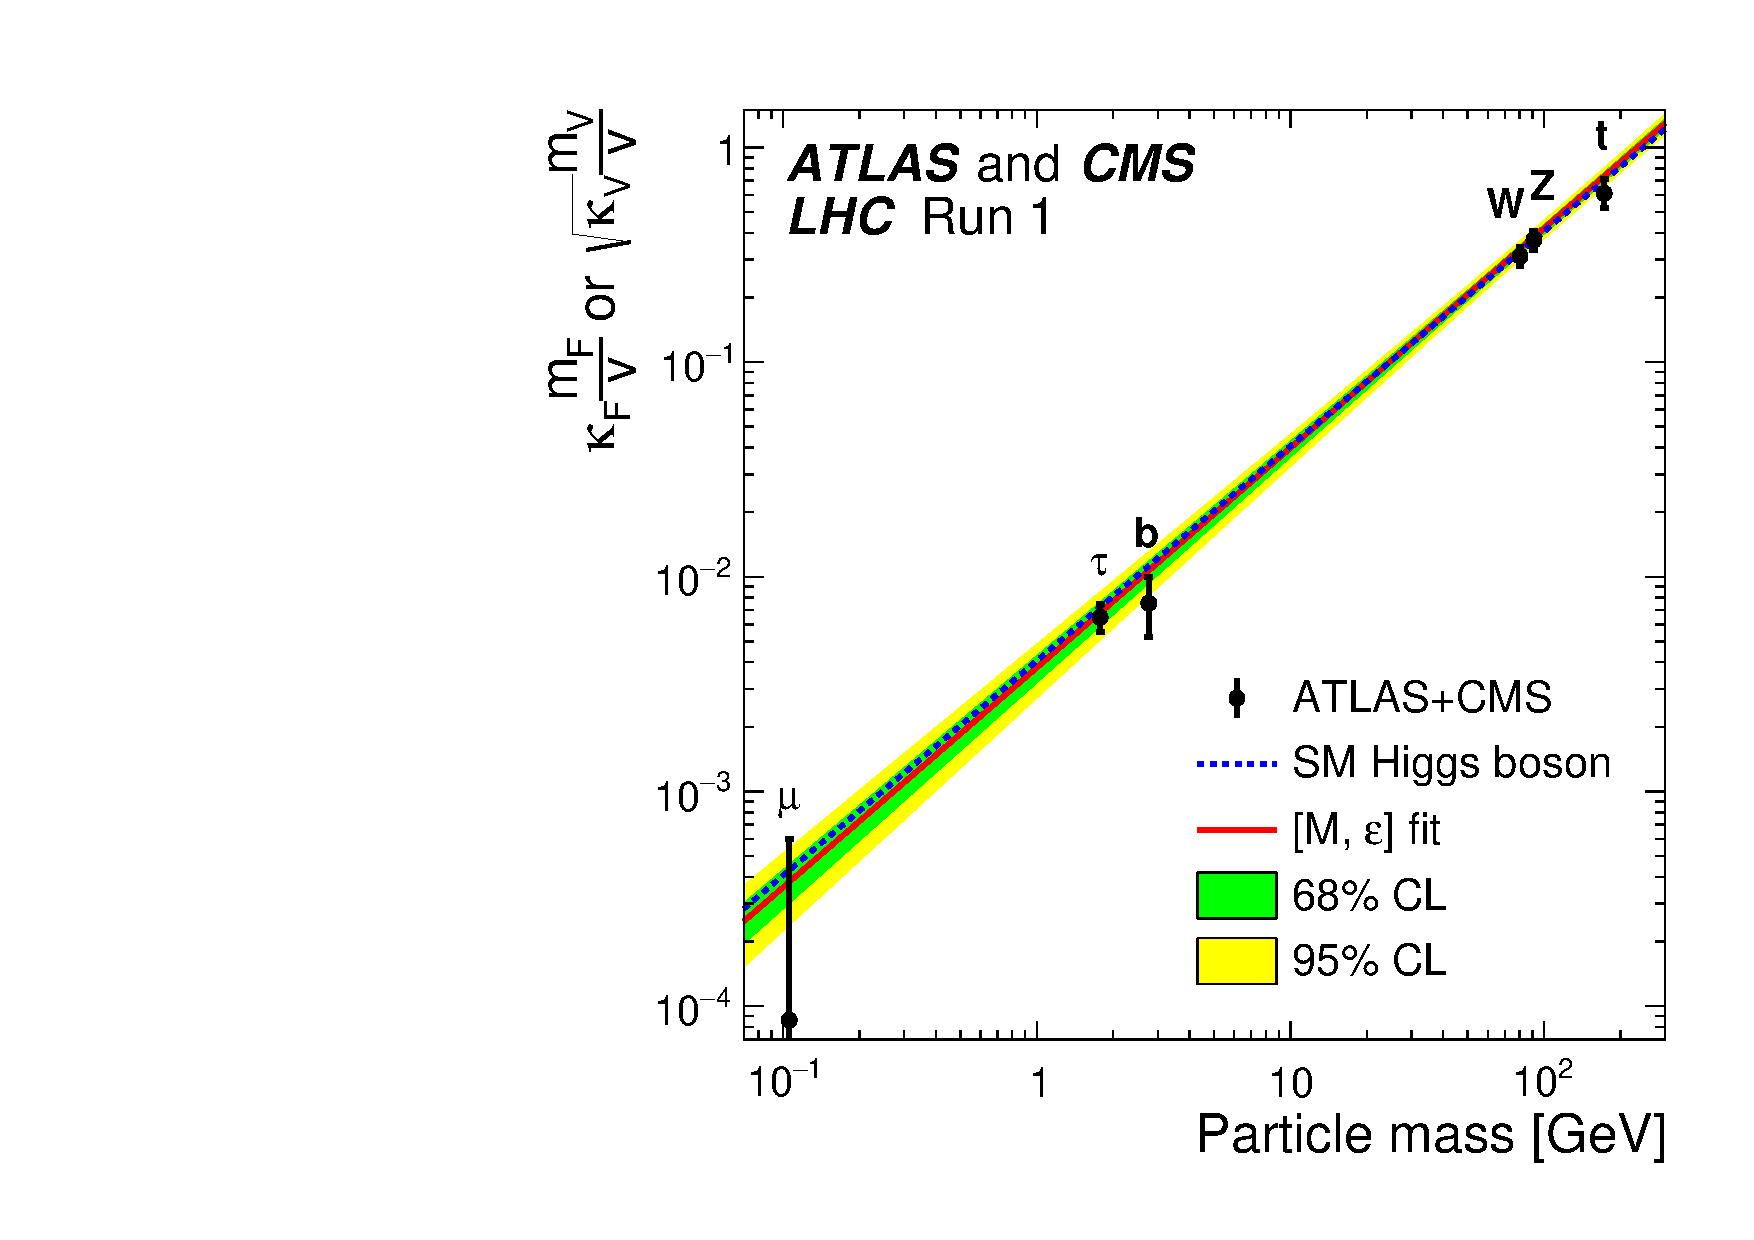
\includegraphics[width=.5\textwidth]{Theory/Meps_lhc.pdf}
\caption{The normalized coupling constants as a function of particle mass for the combination of ATLAS and CMS data~\cite{HiggsProperties}.}
\label{fig:HiggsCouplingMeasurement}
\end{figure}


\section{Higss Boson Pair Production}

The measurement of HH production is a vital test of the SM. However, at $\sqrt{s}=13$ TeV the HH production cross section, $\sigma_{\mathrm{HH}}$, is only ${\sim}35$ fb, about 1000 times smaller than SM Higgs production cross sections, making this measurement extremely challenging and possibly not doable during the planned lifetime of the LHC. To further impede the measurement of $\lambda_{\mathrm{HHH}}$, there are two types of HH production: resonant and non-resonant. Resonant processes contain triHiggs vertices and therefore access this coupling, while non-resonant signals are typically produced when both Higgs couple to vector bosons or heavy quarks. Disentangling resonant and non-resonant production further reduces the sensitivity of HH searches to $\lambda_{\mathrm{HHH}}$. However, there are many BSM theories that predict an enhancement to the HH signal and it is necessary to conduct HH searches to verify that BSM physics is not involved in electroweak symmetry breaking. 


\subsection{Standard Model Production}
At the LHC, there are five main processes that contribute to HH production: gluon fusion, vector boson fusion, double Higgs-strahlung, and top pair and single top production in association with HH production. The cross section for these process can be seen in Table~\ref{tab:DiHiggsXsec} for a center of mass energy of 13 and 14 TeV. Gluon fusion is the leading production mechanism and the two leading diagrams for this process are in Figure~\ref{fig:GF_DiHiggs}. These diagrams have quark loops in them that are dominated by top quarks. Therefore, the cross section for this process depends on $\lambda_{\mathrm{HHH}}$ and the top quark Yukawa coupling. Also, these diagrams interfere destructively causing the low production cross section. This makes searches for HH production intriguing since any observation would be a clear indication of BSM physics.



\begin{table}[h!]
\renewcommand{\arraystretch}{1.5}
\begin{center}
%    \begin{tabular}{l|cc|cc|cc}
    \begin{tabular}{l c c}
% the header
        \hline
        \hline
%         & \multicolumn{2}{c|}{$\sqrt s = 8 $TeV}
         & $\sqrt s = 13 $ TeV & $\sqrt s = 14 $ TeV \\
  %       & \multicolumn{2}{c}{$\sqrt s = 14 $TeV}\\
%         & \multicolumn{2}{c|}{ (LO) NLO} 
%         & \multicolumn{2}{c|}{ NLO} \\
%         & \multicolumn{2}{c}{ (LO) NLO}               \\
         \hline
         Gluon Fusion & 
%$(5.44 ^{+38\%}_{-26\%})  $&$ 8.73 ^{+17 +2.9\%}_{-16 -3.7\%} $ & 
$   33.49 ^{+4.3 +2.1 +2.3\%}_{-6.0 -2.1 -2.3\%} $ & $   39.59^{+4.4 +2.1 +2.2\%}_{-6.0 -2.1 -2.2\%} $ \\
%$(22.8 ^{+32\%}_{-23\%}) $&$   34.8^{+15 +2.0\%}_{-14 -2.5\%} $\\ 
         Vector Boson Fusion  & 
%$ (0.436 ^{+12 \%}_{-10 \%}) $&$ 0.479 ^{+1.8 +2.8\%}_{-1.8 -2.0\%} $ & 
$ 1.62 ^{+2.3+2.3\%}_{-2.7 -2.3\%} $ & $ 1.95 ^{+1.8+2.4\%}_{-2.3 -2.4\%} $\\ 
%$ (1.839 ^{+8.9 \%}_{-7.7 \%})  $&$  2.017 ^{+1.3 +2.5\%}_{-1.0 -1.9\%} $\\ 
$ t\bar t HH $ & 
%$ (0.265 ^{+41 \%}_{-27 \%}) $&$ 0.177 ^{+4.7 +3.2\%}_{-19 -3.3\%} $ & 
$ 0.772 ^{+1.7 +3.2\%}_{-4.5 -3.2\%} $ & $ 0.949 ^{+1.8 +3.2\%}_{-4.8 -3.2\%} $\\
%$ (1.245 ^{+36 \%}_{-25 \%}) $&$ 0.981 ^{+2.3 +2.3\%}_{-9.0 -2.8\%} $\\ 
$ ZHH $ & 
%$ (0.098 ^{+4.2 \%}_{-4.0 \%}) $&$ 0.130 ^{+2.1 +2.2\%}_{-1.9 -1.9\%} $ & 
$ 0.362 ^{+3.4 +1.9\%}_{-2.6 -1.9\%} $ & $ 0.414 ^{+3.5 +1.8\%}_{-2.7 -1.8\%} $ \\
%$ (0.273 ^{+1.1 \%}_{-1.3 \%}) $&$ 0.356 ^{+1.7 +1.9\%}_{-1.2 -1.5\%} $\\ 
$ W^+ HH $ & 
%$ (0.111 ^{+4.0\%}_{-3.9 \%}) $&$ 0.145 ^{+2.1 +2.5\%}_{-1.9 -1.9\%} $ & 
$ 0.329 ^{+0.32 +2.2\%}_{-0.41 -2.2\%} $ & $ 0.368 ^{+0.33 +2.1\%}_{-0.39 -2.1\%} $ \\
%$ (0.283 ^{+1.1 \%}_{-1.3 \%}) $&$ 0.364 ^{+1.7 +2.1\%}_{-1.1 -1.6\%} $\\ 
$ W^-HH $ & 
%$ (0.051 ^{+4.2 \%}_{-4.0 \%}) $&$ 0.069 ^{+2.1 +2.6\%}_{-1.9 -2.2\%} $ & 
$  0.173 ^{+1.2 +2.8\%}_{-1.3 -2.8\%} $ & $  0.197 ^{+1.2 +2.7\%}_{-1.3 -2.7\%} $ \\
%$ (0.152 ^{+1.1 \%}_{-1.4 \%}) $&$  0.201 ^{+1.7 +2.2\%}_{-1.1 -1.8\%} $\\ 
$ tjHH $ & 
%$ (5.057 ^{+2.0 \%}_{-3.2 \%}) $&$ 5.606 ^{+4.4 +3.9\%}_{-2.3 -4.2\%} $ & 
$ 0.0281 ^{+5.2 +4.5\%}_{-3.2 -4.5\%} $ & $ 0.0364 ^{+3.7 +4.7\%}_{-1.3 -4.7\%} $ \\
%$ (28.79 ^{+0.0 \%}_{-1.2 \%}) $&$ 37.27 ^{+4.7 +2.6\%}_{-2.7 -3.0\%} $\\ 
\hline
\hline
\end{tabular}

    \caption{\label{tab:one} Cross sections (in fb) for the seven largest Higgs pair production channels at the LHC, with $\sqrt{s} = 13$ and 14 TeV. The first uncertainty is the scale uncertainty, the second is the PDF uncertainty, and the third for gluon fusion is the $\alpha_{s}$ uncertainty. The gluon fusion, $ZHH$, and $W^{\pm}HH$ channels have been calculated at next-to-next-to-leading-order (NNLO) QCD and the vector boson fusion, $ttHH$, and $tjHH$ channels have been calculated at next-to-leading-order (NLO) QCD~\cite{DiHiggsXsec}.}
\label{tab:DiHiggsXsec}
\end{center} 
\end{table}

\begin{figure}[h!]
\begin{center}
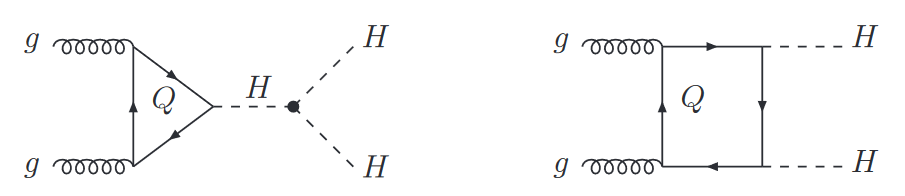
\includegraphics[width=5 in]{Theory/SMdiHiggs_GF.png}
\end{center}
\caption{The two leading HH production diagrams for gluon fusion~\cite{DiHiggsTheory}.}
\label{fig:GF_DiHiggs}
\end{figure}


\subsection{Beyond the Standard Model Production}

The HH signature is theoretically predicted by numerous BSM scenarios and can be observed in two distinct signatures, resonant and non-resonant. A resonant signature would manifest as an enhancement of $\sigma_{\mathrm{HH}}$ at a specific resonance mass, $m_{X}$. A non-resonant signature would produce an overall enhancement of $\sigma_{\mathrm{HH}}$ across a wide range of $m_{X}$ values. Since this thesis describes a search for resonant production, this section will only focus on resonant BSM production. 

The BSM theories that predict the existence of a new resonance $X$ decaying to a pair of Higgs bosons allow for a wide range of possible masses. This range spans from the kinematic limit, which is twice the Higgs mass, up to several TeV. Due to this large range, different search techniques must be employed to completely cover it. This analysis is a model independent search for a heavy resonance, mass just below a TeV up to a couple TeV, and therefore this section will focus on BSM theories that predict these types of particles. This section is not meant to be a complete description of every BSM model that predicts this HH signature, but rather an illustration that this search is well motivated many different types of theories. 

\begin{itemize}[wide, labelwidth=!, labelindent=0pt]
\setlength{\itemindent}{-.9em}
\item[ ]
\textbf{Warped extra dimensions}

\indent
In order to solve the hierarchy problem, the large discrepancy between the weak force and gravity, Randall and Sundrum~\cite{RS} proposed a warped extra dimension (WED) model where there is one extra spatial dimension compactified between two fixed points, called branes. The region between the branes is referred to as bulk and controlled through an exponential metric. The gap between the two fundamental scales of nature, such as the Planck scale ($M_{Pl}$) and the electroweak scale, is controlled by a warp factor, $k$, in the metric, which corresponds to one of the fundamental parameters of the theory. One of the branes, where the density of the extra dimensional metric is localized, is called the ``Planck brane'', while the other, where the Higgs field is localized, is called the ``TeV brane''. This type of model predicts the existence of new particles, such as the spin-0 radion~\cite{Radion, Radion2, Radion3} and the spin-2 first Kaluze-Klein (KK) excitation of the graviton~\cite{Graviton, Graviton2, Graviton3}. 

There are two possible ways of describing a KK graviton, which is the mediator of the gravitational force, from the standpoint of a WED that depends on the choice of localization of the SM matter fields. In the RS1 model, only gravity is allowed to propagate in the extra-dimensional bulk, and the couplings of the KK graviton to matter fields are fully defined by $k/\overline{M}_{Pl}$, where $\overline{M}_{Pl}\equiv M_{Pl}/\sqrt{8\pi}$. If other fields are allowed to propagate in the bulk, the bulk RS model, the coupling of the KK graviton to matter depends on the localization of the SM fields in the bulk. This model is favorable because only the Higgs is on the TeV brane which allows high energy unification of gauge couplings and a natural mass hierarchy. For example, the light quarks are localized near the Planck brane while the top quarks are localized near the TeV brane, the elementary top hypothesis, causing a large top mass.

The radion is an additional element of WED models that is needed to stabilize the size of the extra dimension $l$ and the radion's properties are similar between the two WED models. It is standard to express the benchmark points of the radion in terms of the dimensionless quantity $k/\overline{M}_{Pl}$, and the mass scale $\Lambda_{R} = \sqrt{6} e^{-kl}\overline{M}_{Pl}$, with the latter interpreted as the ultraviolet cutoff of the theory~\cite{WEDuvCutoff}. The addition of a scalar-curvature term can induce a mixing between the scalar radion and Higgs boson~\cite{RadionHMixing}, but due to electroweak precision tests this mixing is expected to be small.

In proton-proton collisions at the LHC, the KK graviton and radion are produced primarily through gluon-gluon fusion. The KK gravition is predicted to decay to a pair of Higgs with a branching fraction of up to ${\sim}10\%$ depending on the type of model and model parameters. While the radion has an HH branching fraction of ${\sim}25\%$ that is roughly constant across models. The absolute value for the production cross section scales with $(k/\overline{M}_{Pl})^{2}$ for the KK gravition~\cite{GravitionXS} and with $1/\Lambda_{R} ^{2}$ for the radion~\cite{RadionXS}. 

\item[ ]
\textbf{Higgs singlet}

\indent
The simplest extension of the SM Higgs sector is done by adding a real singlet field, S~\cite{HiggsSinglet}. The scalar potential is then

\begin{equation}
V(\Phi,S)= -m^{2}\Phi^{\dag}\Phi -\mu^{2}S^{2}+\lambda_{1}(\Phi^{\dag}\Phi)^{2}+\lambda_{2}S^{4}+\lambda_{3}\Phi^{\dag}\Phi S^{2}
\end{equation}

\noindent
where $\Phi$ is the complex scalar doublet of $SU(2)$ from the SM. In the unitary gauge, the Higgs fields are given by

\begin{equation}
\Phi = 
\begin{pmatrix}
0\\
\frac{\widetilde{h}-\nu}{\sqrt{2}}
\end{pmatrix},
\end{equation}

\begin{equation}
S= \frac{h^{\prime}+x}{\sqrt{2}}
\end{equation}

\noindent
where $\nu$ and $x$ are the vacuum expectation values for the $\Phi$ and $S$ fields, respectively. The gauge and mass eigenstates are then related by the mixing matrix

\begin{equation}
\begin{pmatrix}
h\\
H
\end{pmatrix}
= 
\begin{pmatrix}
\mathrm{cos}\: \alpha & -\mathrm{sin}\: \alpha \\
\mathrm{sin}\: \alpha & \mathrm{cos}\:\alpha
\end{pmatrix}
\begin{pmatrix}
\widetilde{h}\\
h^{\prime}
\end{pmatrix}
\end{equation} 

\noindent
where h represents the SM Higgs and H is a new, additional Higgs. The free parameters in this model are $m_{h}$, $m_{H}$, $\mathrm{sin}\:\alpha$, $\nu$, and $x$. When $m_{H} > 2m_{h}$, the $H\rightarrow hh$ decay is allowed and the second Higgs is decoupled from other SM particles~\cite{HiggsSingletPheno}. In this scenario, the second Higgs is primarily produced through gluon fusion and can have a mass from $250-1000$ GeV. The branching fraction of $H$ to two SM Higgs is up to $40\%$ depending on the parameters of the model.

\item[ ]
\textbf{Georgi-Machacek model}

\indent
The Georgi-Machacek (GM) model~\cite{GMmodel} is a more complicated extension of the Higgs sector where a real triplet field, $\xi$, with hypercharge $Y=0$ and a complex $SU(2)_{L}$ triplet field, $\chi$, with hypercharge $Y=1$ are added. This is an interesting model because the triplet fields can have vacuum expectation values which leads to neutrinos having light Majorana masses. The model also predicts the existence of three neutral scalars, two that are CP-even and one that is CP-odd. At the LHC, the production of one of these CP-even scalars is dominated by gluon fusion. This scalar can be as heavy as 1 TeV and it decays to a pair of Higgs bosons with a branching fraction that can be as large as ${\sim}95\%$ depending on the mass of the scalar. The GM model has the intriguing phenomenological feature that the couplings between the SM Higgs and the SM weak gauge bosons are enhanced, meaning that precision measurements of Higgs couplings could also give evidence to this model~\cite{GMmodelPheno}.


\end{itemize}

%\section{DiHiggs Phenomenology}














